\section{Superfici}

\begin{definition}[Superficie regolare]
Sia $D \subseteq \mathbb{R}^2$ un dominio \underline{connesso}. Una funzione $\varphi : D \to \mathbb{R}^3$ si dice \underline{superficie regolare} se:
\begin{enumerate}
    \item $\varphi \in C^1(D)$;
    \item $\varphi|_{\mathring{D}}$ è \underline{invertibile};
    \item $\forall (u, v) \in \mathring{D}$, scrivendo $\varphi(u, v) = (\varphi_1(u, v), \varphi_2(u, v), \varphi_3(u, v))$, la matrice jacobiana
    \[
    \frac{\partial(\varphi_1, \varphi_2, \varphi_3)}{\partial(u, v)}
    = \begin{pmatrix}
    \dfrac{\partial \varphi_1}{\partial u} & \dfrac{\partial \varphi_1}{\partial v} \\[10pt]
    \dfrac{\partial \varphi_2}{\partial u} & \dfrac{\partial \varphi_2}{\partial v} \\[10pt]
    \dfrac{\partial \varphi_3}{\partial u} & \dfrac{\partial \varphi_3}{\partial v}
    \end{pmatrix}
    = \big(\, \varphi_u \ \big|\ \varphi_v \,\big)
    \]
    ha \underline{rango $2$}, ovvero almeno uno dei seguenti determinanti minori è non nullo:
    \[
    A = \begin{vmatrix}
    \dfrac{\partial \varphi_1}{\partial u} & \dfrac{\partial \varphi_1}{\partial v} \\[8pt]
    \dfrac{\partial \varphi_2}{\partial u} & \dfrac{\partial \varphi_2}{\partial v}
    \end{vmatrix}, \qquad
    B = \begin{vmatrix}
    \dfrac{\partial \varphi_2}{\partial u} & \dfrac{\partial \varphi_2}{\partial v} \\[8pt]
    \dfrac{\partial \varphi_3}{\partial u} & \dfrac{\partial \varphi_3}{\partial v}
    \end{vmatrix}, \qquad
    C = \begin{vmatrix}
    \dfrac{\partial \varphi_1}{\partial u} & \dfrac{\partial \varphi_1}{\partial v} \\[8pt]
    \dfrac{\partial \varphi_3}{\partial u} & \dfrac{\partial \varphi_3}{\partial v}
    \end{vmatrix}
    \]
\end{enumerate}
Equivalentemente, la condizione (3) si esprime come:
\[
A^2 + B^2 + C^2 > 0 \qquad \text{in } \mathring{D}
\]
Le equazioni parametriche della superficie sono:
\[
\begin{cases}
x = \varphi_1(u, v) \\
y = \varphi_2(u, v) \\
z = \varphi_3(u, v)
\end{cases}
\qquad (u, v) \in D
\]
\end{definition}

\begin{definition}[Piano tangente e versore normale]
Il piano passante per $\varphi(u, v)$ individuato dai vettori linearmente indipendenti $\varphi_u(u, v)$ e $\varphi_v(u, v)$ si chiama \underline{piano tangente} alla superficie nel punto $\varphi(u, v)$.

Il vettore prodotto vettoriale $\varphi_u \wedge \varphi_v$ ha modulo
\[
|\varphi_u \wedge \varphi_v| = \sqrt{A^2 + B^2 + C^2} > 0
\]
Si definisce \underline{versore normale} alla superficie il vettore unitario
\[
N(u, v) = \frac{\varphi_u \wedge \varphi_v}{|\varphi_u \wedge \varphi_v|} \qquad \text{\pencilnote{(altra notazione: $\nu(u, v)$)}}
\]

\begin{center}
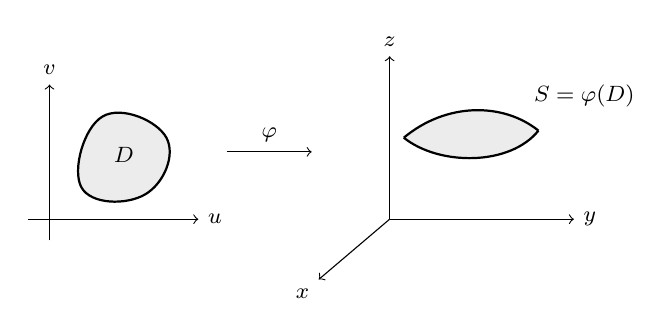
\begin{tikzpicture}[scale=0.9]
    % Piano (u, v)
    \begin{scope}[shift={(-3.0,0)}]
        \draw[->] (-0.3,0) -- (2.1,0) node[right] {\footnotesize $u$};
        \draw[->] (0,-0.3) -- (0,1.9) node[above] {\footnotesize $v$};
        \fill[gray!15] plot[smooth cycle, tension=0.8] coordinates {
            (0.45,0.45) (1.35,0.35) (1.65,1.15) (0.75,1.45)
        };
        \draw[thick] plot[smooth cycle, tension=0.8] coordinates {
            (0.45,0.45) (1.35,0.35) (1.65,1.15) (0.75,1.45)
        };
        \node at (1.05,0.9) {\footnotesize $D$};
    \end{scope}

    % Freccia mappa phi
    \draw[->] (-0.5,0.95) -- (0.7,0.95) node[midway, above] {\footnotesize $\varphi$};

    % Spazio R^3 e superficie S = phi(D)
    \begin{scope}[shift={(1.8,0)}]
        \draw[->] (0,0) -- (2.6,0) node[right] {\footnotesize $y$};
        \draw[->] (0,0) -- (0,2.3) node[above] {\footnotesize $z$};
        \draw[->] (0,0) -- (-1.0,-0.85) node[below left] {\footnotesize $x$};

        % Calotta S = phi(D)
        \fill[gray!15] (0.2,1.15)
            .. controls (0.8,1.65) and (1.6,1.65) .. (2.1,1.25)
            .. controls (1.7,0.75) and (0.7,0.75) .. (0.2,1.15);
        \draw[thick] (0.2,1.15) .. controls (0.8,1.65) and (1.6,1.65) .. (2.1,1.25);
        \draw[thick] (0.2,1.15) .. controls (0.7,0.75) and (1.7,0.75) .. (2.1,1.25);
        \node[above right] at (1.9,1.45) {\footnotesize $S = \varphi(D)$};
    \end{scope}
\end{tikzpicture}
\end{center}
\end{definition}

\begin{esercizio}[Esempio 1 -- Superfici cartesiane]
Sia $f : D \subseteq \mathbb{R}^2 \to \mathbb{R}$, con $f \in C^1(D)$ e $D$ dominio connesso. Si chiama \underline{superficie cartesiana} la superficie parametrizzata da:
\[
\varphi : \begin{cases}
x = u \\
y = v \\
z = f(u, v)
\end{cases}
\qquad (u, v) \in D
\]
Calcolando le derivate parziali:
\[
\varphi_u = (1, 0, f_u(u, v)), \qquad \varphi_v = (0, 1, f_v(u, v))
\]
si ha
\[
|\varphi_u \wedge \varphi_v|^2 = f_u^2 + f_v^2 + 1 = 1 + |\nabla f|^2 > 0
\]
Quindi ogni superficie cartesiana di classe $C^1$ è sempre regolare.
\end{esercizio}

\begin{esercizio}[Esempio 2 -- Superfici cilindriche]
Sia $\gamma : [a, b] \to \mathbb{R}^2$ una curva regolare e semplice, con equazioni parametriche
\[
\begin{cases}
x = x(t) \\
y = y(t)
\end{cases}
\qquad t \in [a, b]
\]
La superficie parametrizzata su $D = [a, b] \times [z_1, z_2]$ da
\[
\varphi : \begin{cases}
x = x(t) \\
y = y(t) \\
z = z
\end{cases}
\qquad t \in [a, b], \ z \in [z_1, z_2]
\]
\pencilnote{(notazione leggermente ambigua per il doppio ruolo di $z$)} si dice \underline{superficie cilindrica}.

\begin{center}
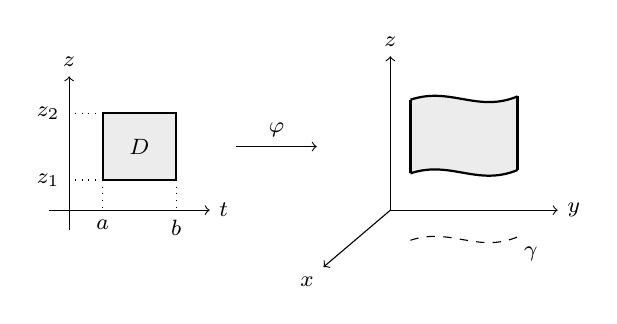
\begin{tikzpicture}[scale=0.85]
    % Rettangolo dei parametri [a, b] x [z_1, z_2]
    \begin{scope}[shift={(-3.1,0)}]
        \draw[->] (-0.3,0) -- (2.1,0) node[right] {\footnotesize $t$};
        \draw[->] (0,-0.3) -- (0,2.0) node[above] {\footnotesize $z$};
        \fill[gray!15] (0.5,0.45) rectangle (1.6,1.45);
        \draw[thick] (0.5,0.45) rectangle (1.6,1.45);
        \draw[dotted] (0.5,0.45) -- (0.5,0) node[below] {\footnotesize $a$};
        \draw[dotted] (1.6,0.45) -- (1.6,0) node[below] {\footnotesize $b$};
        \draw[dotted] (0.5,0.45) -- (0,0.45) node[left] {\footnotesize $z_1$};
        \draw[dotted] (0.5,1.45) -- (0,1.45) node[left] {\footnotesize $z_2$};
        \node at (1.05,0.95) {\footnotesize $D$};
    \end{scope}

    \draw[->] (-0.6,0.95) -- (0.6,0.95) node[midway, above] {\footnotesize $\varphi$};

    % Superficie cilindrica in R^3
    \begin{scope}[shift={(1.7,0)}]
        \draw[->] (0,0) -- (2.5,0) node[right] {\footnotesize $y$};
        \draw[->] (0,0) -- (0,2.3) node[above] {\footnotesize $z$};
        \draw[->] (0,0) -- (-1.0,-0.85) node[below left] {\footnotesize $x$};

        % Curva base gamma sul piano xy
        \draw[dashed] (0.3,-0.45) .. controls (0.9,-0.25) and (1.3,-0.65) .. (1.9,-0.4);
        \node[below right] at (1.85,-0.4) {\footnotesize $\gamma$};

        % Striscia cilindrica
        \fill[gray!15] (0.3,0.55)
            .. controls (0.9,0.75) and (1.3,0.35) .. (1.9,0.6)
            -- (1.9,1.7)
            .. controls (1.3,1.45) and (0.9,1.85) .. (0.3,1.65)
            -- cycle;
        \draw[thick] (0.3,0.55) .. controls (0.9,0.75) and (1.3,0.35) .. (1.9,0.6);
        \draw[thick] (0.3,1.65) .. controls (0.9,1.85) and (1.3,1.45) .. (1.9,1.7);
        \draw[thick] (0.3,0.55) -- (0.3,1.65);
        \draw[thick] (1.9,0.6) -- (1.9,1.7);
    \end{scope}
\end{tikzpicture}
\end{center}

Calcolando le derivate parziali rispetto a $t$ e $z$:
\[
\varphi_t = (x'(t), y'(t), 0), \qquad \varphi_z = (0, 0, 1)
\]
si ottiene:
\[
|\varphi_t \wedge \varphi_z|^2 = \big(y'(t)\big)^2 + \big(x'(t)\big)^2 = |\gamma'(t)|^2 > 0
\]
poiché $\gamma$ è regolare. Inoltre $\varphi_t \wedge \varphi_z = (y'(t), -x'(t), 0)$, da cui il versore normale alla superficie cilindrica è:
\[
N(t, z) = \frac{\varphi_t \wedge \varphi_z}{|\varphi_t \wedge \varphi_z|} = \left( \frac{(y'(t), -x'(t))}{|\gamma'(t)|},\, 0 \right) = (N_\gamma(t), 0)
\]
\end{esercizio}